\section{Bases de données}
Les trois bases de données qui ont été analysées pour les fins du présent travail sont la \texttt{norwegianfire} et \texttt{Secura} du package \texttt{R Reins} ainsi que \texttt{Danish} du package \texttt{QRM}. Elles ont en commun qu'elles comportent toutes des montants extrêmes, ce qui les rend intéressantes pour l'étude des queues de distribution épaisses. En voici donc une courte description. D'ailleurs, elles ont été l'objets d'études dans le domaine de la réassurance dont les résultats ont été publiés dans(...) \cite{norwegianfireEtSecura} et \cite{Danish}

	\subsection{Norwegianfire}
	Cette base de données est accessible via la commande \texttt{R} \texttt{data("norwegianfire")} ou via le lien suivant: \url{http://lstat.kuleuven.be/Wiley}. Il s'agit d'une compilation des réclamations relatives aux incendies de forêt ayant eu lieu en Norvège pendant la période de 1972 à 1992.\\ 
	
	À la lecture de ces données, il est important d'observer que les réclamations retenues sont supérieures à 500 000 couronnes norvégiennes. Ce qui fait en sorte qu'il faut conditionner sur les lois de probabilité afin de bien tenir compte de cette troncature.\\
	
	À noter qu'aucune mention n'a été faite au sujet d'un éventuel ajustement pour l'inflation. Dans le cadre de ce travail, nous présumerons qu'un ajustement a été fait.
	
		%\paragraph{Analyse préliminaire}
			%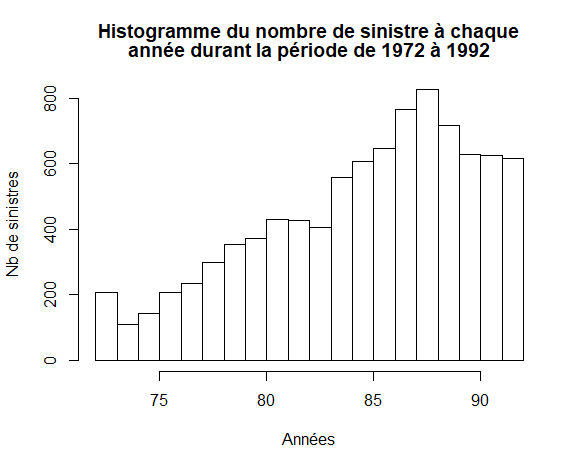
\includegraphics{Graphiques/HistFreqNorwegianfire}
	
	\subsection{Secura}
	Toujours dans le package \texttt{Reins}, cette base de données comporte des montants de réclamation en assurance automobile venant de plusieurs pays d'Europe pendant la période de 1988 à 2001. Ces montants sont en excédant de 1\,200\,000 euros et sont ajustées pour l'inflation.
	
	\subsection{Danish}
	Cette dernière base de données peut être trouvée dans le package \texttt{R QRM} ou au lien suivant: \url{http://www.ma.hw.ac.uk/~mcneil/data.html}. Elle a été compilée à la Copenhagen Reinsurance et comprend 2\,167 pertes liées à des incendies au cours de la période de 1980 à 1990. Elle a été ajusté pour inflation et est exprimée en millions de couronnes danoises.	De plus, aucune troncature n'a été faite sur les données; il n'est donc pas nécessaire de conditionner dans ce cas-ci.\\
	
	Par ailleurs, ce qui distingue cette base de données des deux autres, c'est qu'elle présente les sinistres à chaque jour. Il est donc possible d'avoir une analyse de la fréquence plus approfondie.
	